% !TeX root = ../main.tex
% Add the above to each chapter to make compiling the PDF easier in some editors.

\chapter{Approach}\label{chap:approach}

The proposed system is a "breathable" distributed system, where breathable means that it can react at runtime to distinct situations to reconfigure itself and update a decision of where the tasks will execute, always prioritizing the execution of tasks based on their criticality. The situations that trigger this breathable behavior are mainly categorized in two types: 1) changes to the set of tasks that the system must execute (task queue) and 2) changes to the availability of computing resources. In the first category, it is assumed that all tasks have at least soft real-time behavior and they can all be categorized as periodic (need to be executed every certain time period) or sporadic (are executed upon request and at unpredictable moments) [**add reference**]. In the scope of this work and for simplicity, we assume two generalizations: a) all tasks can be treated as periodic tasks with a variable number of jobs (individual executions of the task that can be repeated), where specific cases with 1 total job represent sporadic tasks and an infinite number of jobs represent common periodic tasks, which could be split in batches of jobs for less critical tasks; and b) all tasks can be migrated from one device to another in between jobs. Furthermore, in the scope of this work it is assumed that tasks have no data or sequential dependencies with each other. The second category includes reacting to addition or removal of physical devices or hardware (for example, due to hardware failure or device restarts triggered by updates, etc.) and also to the availability and latency of virtual devices in the mobile-edge-cloud (for example, when driving over a highway section with MEC support).

These characteristics of the system can be summarized in the image below (add proper reference). The system behavior can be then described as follows. First, a reconfiguring situation triggers a re-distribution of the tasks that need to be executed, which are kept in the global queue. This global task queue as well as the set of both physical and virtual devices (or ECUs) are fed to a task partitioning algorithm, which decides a task-to-board mapping and then triggers the distribution of the tasks on the respective mapped device. The final step is that, depending on the previous mapping of tasks to boards, if the assigned ECU for a task changes, it is necessary to migrate its execution from the previous device (source) to the new one (target). This last step is the main objective of this research work, and in the scope of it, a few requirements should be considered to deem the implementation as successful: 1) the task has to be stopped in the source device and started in the target device, 2) the relevant task context should be also migrated, meaning that no crucial data is lost (in the case of a SLAM algorithm, the map and position would not be lost), 3) both the migration decision and execution strategies should consider the criticality of the tasks, 4) real-time behavior should be also considered in the migration strategy. It is relevant to mention that a master ECU would be responsible for both keeping the global task queue, triggering the task-to-board distribution algorithm (which itself can run on a separate ECU or a specialized ML hardware) and keeping the relevant files to start tasks when necessary.
 

\begin{center}
	\makebox[\textwidth]{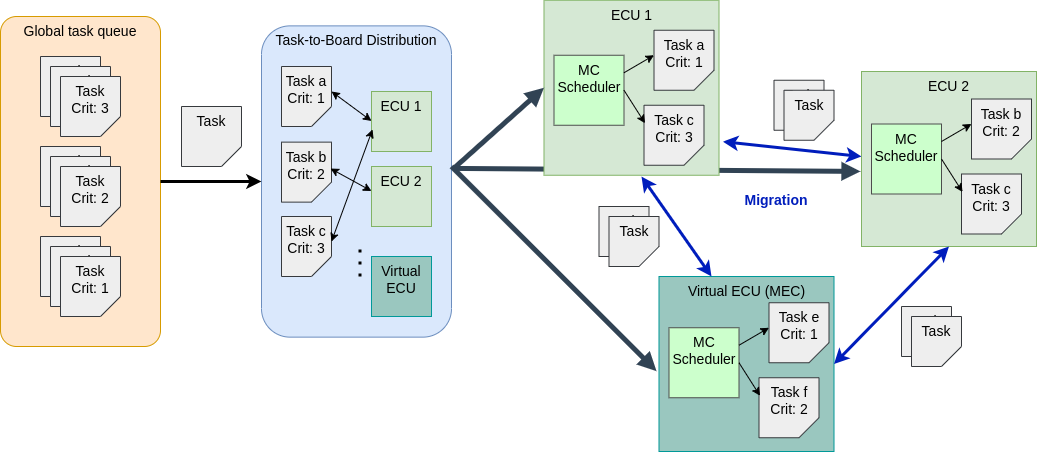
\includegraphics[width=\textwidth]{figures/Migration_Diag_new.png}}
\end{center}

Based on the previous list of requirements, and especially 3 and 4, at least 2 migration strategies should be implemented, since tasks with different criticalities also have different constraints to be prioritized. For example, in the case of low-criticality tasks, it might be more relevant that the task does not end in starvation, whereas for a high critical task it is crucial that the result is delivered always on-time and that, if the task needs to be paused due to a critical failure, it is brought back up in a minimal and deterministic time to keep up with the real-time constraints.

\subsection{Contributions}
This is just conceptually speaking... But in order to better place my contribution

\begin{itemize}
	\item Task-to-Board distribution/migration planning: Toolchain for integrating ML was result of Bernhard + Robert Hamsch's thesis. My contribution: adaption to my embedded devices + include ECU, adaption to send ELF files + checkpoints, adaption to keep PTP synchronization
	\item ECU base system (OS): Selection of FreeRTOS as base RTOS (Bernhard, probably with input from Oliver), confirmed by me. Decision of AMP over SMP in multicore case (Bernhard + me). Some inter-processor features (probably Oliver + students). My contribution: extension of ESFREE to include MC (supported by students Mahdi and Kamran). Conceptual architecture of ELF loader, wrapper task, checkpoint keeping (implementation Yinbo).
	\item Guest task architecture: My contribution (supported by results of Yinbo): C task architecture in form of a library + simplified linker script (adapted from Yinbo's thesis)
	\item Migration strategy HI: My contribution: concept definition. Implementation partially shown in PoC by Dorota, must be extended still + maybe will require distributed shared memory implementation?
	\item Migration strategy LO: Concept definition (me) + implementation and PoC by Yinbo
	\item Migration strategy Virtual ECU (LO): Concept definition (me + Bernhard) + partial implementation and PoC analysis by Roberto + adaption and integration (me + probably Mahdi)
	\item Further system features: PTP + SOMEIP (Yinbo implementation + me/Bernhard concept), strategy for system functions (me), missing - network, other peripherals, interrupts, mem management? 
\end{itemize}


\section{General Overview}\label{section:descriptionapproach}

As mentioned before, the main objective of the proposed research is to achieve the integration of mixed criticality into the task migration process. The proper integration would require different strategies for the different criticality modes. For this reason, it is first important to define what is understood under mixed criticality in the scope of this work. While many publications consider only two criticality levels (high and low), the standards commonly describe several of them. In this work, the concept of multiple criticality levels will be used in a conceptual phase following the ASIL standard in ISO 26262, while the implementation and results will be collected for at least 2 levels in both the scheduling algorithm and the migration strategy. Whereas a model with multiple criticality levels represents real situations better over one with just two, as tasks can have intermediate criticality levels, in the scope of this work, the focus relies more on fulfilling challenges at both ends of the criticality spectrum, and assuming a mix of both strategies might apply as a solution for intermediate levels. One concept that should be covered is the consideration of different execution times according to a criticality level, as normally higher criticality levels offer pessimistic WCET estimates to ensure correct behavior occurs, but actual execution times are often lower. This is a concept that is explored in many publications and is often necessary to ensure compliance with certification authorities.

The first element needed for the system developed is the integration of a mixed-criticality scheduler for each of the physical devices. This should ensure that for any given device, the tasks with a higher criticality will never miss the deadline for a job, while being more flexible for lower criticality levels. In this regard, exploring different mixed-criticality scheduling algorithms and their integration in the development platform is an important step that will allow the migration to occur and be evaluated properly. Several publications have proposed mixed-criticality scheduling algorithms, such as ~\parencite{baruah1, fleming1, zhao1, baruah2, lili1}, and a few of them can be implemented and compared. It is also important to mention that following the state of the art in embedded devices, a multi-core implementation is desired, with asymmetrical multiprocessing (AMP) being the preferred solution, as software failures could be isolated to affect less tasks (***find a reference***). In particular, following approaches are explored (so far): hierarchical virtual deadline EDF (faulty implementation); reserved cores for 2-level MC, with LO crit cores as backup cores for HI tasks. It is assumed that this step should not affect the behavior of the virtual devices, since by concept, they can only run non highly (not necessarily only LO) critical tasks, due to the uncertainties introduced by the external communication with the MEC (explain further...).

Another important element for the distributed system to ensure its compliance to the real-time constraints is a timing protocol such as PTP, to keep the different devices synchronized and share the same notion of time when following task deadlines. This way, even when migrating a task, information on the deadlines should be very accurate. In addition to this, migration strategies must consider that transmission times can be variable and, in the ideal case, the source device should keep the original task execution until it is ensured that the target device has started the execution successfully, potentially taking longer than the deadline of a running job.

The migration planning will be adapted from previous work, namely the student theses supervised by Bernhard Blieninger. As these don't consider mixed-criticality or a multi-core implementation in the system behavior, a few changes are necessary to integrate both concepts. First, the schedulability analysis that is commonly used for selecting the best task distribution has to be extended to work with criticality levels and the use of a mixed-criticality scheduler. Here, it has to be taken into consideration whether extending and retraining the machine learning models is worth the effort, especially since this idea is still not proven as a solution and the extension with the criticality levels and other relevant information might add complexity to the net. Otherwise, implementing a mathematical schedulability analysis that considers mixed criticality is necessary. A second extension that should be performed in the planning stage is to penalize the migration of higher criticality tasks, as the migration overhead adds an additional risk for the tasks failing. Furthermore, the availability of both virtual and physical devices needs to be considered at the moment of deciding which tasks should migrate and where.

The next step in the development of this strategy is the execution of the migration, which is the core concept explored in this work. It is important to consider the necessity to meet strict timing constraints for tasks at the higher end of the criticality spectrum. ***THIS HI criticality solution is yet to be explored, Yinbo is working on the variant for LO crit*** While the exact approach is yet to be proven as feasible, an idea for higher criticality tasks would be to let them run in a standby state in all or a subset of the total of available ECUs, and only executing it in one ECU, while storing runtime generated data either in a central unit or in a shared memory only accessible to highly critical tasks, in this way only a start/stop signal is sent to the task and the execution can be resumed quickly, also ensuring fail-safety in case the executing device fails. Also, for tasks that require redundancy (e.g. ASIL level D), it should be possible for tasks to execute actively multiple times and produce results in parallel. Another addition in this stage should be the introduction of a real-time capable communication protocol. In this sense, it should be possible to bound the migration time for this tasks, ideally in the range of a few milliseconds. These ideas could be faster to execute and allow for less variance in the time, eventually making it possible to perform formal verification, but it would be expensive if tasks at all criticality levels were to run like that, as the resources are utilized inefficiently. This should be acceptable for highly critical tasks, though, since the majority of the tasks would be assigned low to medium criticality levels.

The strategy for migrating lower criticality tasks between physical devices is prone to more flexibility, so that a wider range of tasks can be deployed with a lower impact in terms of resource efficiency, even if this would open the possibility for more erroneous behavior in the tasks. The approach currently explored for tasks with low criticality involves the transmission of precompiled task binaries and a snapshot of the execution data every time a task is distributed to an ECU and the usage of a normal TCP/IP protocol over Ethernet. ***This is Yinbo's ELF loader thesis*** With this strategy, the resource utilization in the devices is made more efficient, but the time spent for the migration is increased as the communication is slower due to the amount of information exchanged, and also less reliable due to the nature of the communication protocol. 

As an optional step, the exploration of strategies for more criticality levels is yet to be done, but a few ideas are suggested. First, a combination of the two strategies mentioned could be implemented for intermediate criticality levels, such as leaving the tasks running but using a less predictable communication protocol. Another idea is to subdivide each of the criticality levels mentioned and there perform variations of the mentioned strategy. For example, in a system with a certain number of devices and 2 high criticality sublevels, the highest sublevel tasks are kept in standby on all devices, while the rest are only kept in standby in a few of the devices, making sure there is always an ECU ready for the highest criticality and using less resources for the second sublevel. In the case of lower criticality, this could be implemented in the form of giving priority to the migration and transmission of data of tasks at the higher sublevels.

Additionally, due to the consideration of virtual devices in the MEC, an additional strategy is also implemented in the scope of this work. That is, the migration of low criticality tasks from and to the MEC. For this implementation, it is assumed that the MEC servers share some aspects of the architecture with the real hardware and that the devices can be modeled in the form of containers as their digital twins. In this way, upon availability, the master ECU can request to start a container which will run the required task. It is assumed that this behavior is allowed for low criticality tasks that can benefit from the more powerful resources available in the MEC, and that communication latency can be neglected as long as the results produced are relevant. An example of this might be a path planning algorithm for an autonomous vehicle, where the immediate safety of the vehicle is not threatened, but the algorithm can be extended with further sensor data and better hardware for performing ML tasks. ***Part of this has already been implemented by Roberto*** It is relevant in the scope of the migration, that the virtual tasks have an equivalent task implemented for the real devices, and that the task data can also be migrated between them. In this way, the task can be moved depending on the need and availability of the resources to and from the MEC.


\section{Overall System Architecture}

\begin{itemize}
	\item Master ECU responsible for keeping track of global queue list and available hardware. Also responsible for triggering task-to-board distribution and deployment. This master ECU might have a backup ECU to meet requirements and furthermore keeps all relevant data for all tasks (precompiled task binaries / container images, context data files, criticality levels). Current implementation represents master ECU with a more powerful workstation - could be implemented to work on an embedded board similar to the other devices.
	\item Component performing task partitioning algorithm (might be ML-supported schedulability analysis as developed with Bernhard). Assumed to be a "black box" in most of the thesis as it is not in the scope of this research.
	\item Physical ECUs based on a FreeRTOS kernel extended with the functionality needed for the task migration and to comply with MC, as well as resource optimization through multicore. Some of these ECUs might be kept in a hot-standby mode or off to have backup devices while minimizing energy consumption in the vehicle
	\item Virtual ECUs based on a containerized minimal version of the FreeRTOS system that can execute the same tasks without the need for changes in the code
	\item Embedded OS Software Architecture: Extensions to the FreeRTOS Kernel - scheduler, deployment slave, inter-core communication, execution and monitoring of real-time behavior
	\item Task Specific Software Architecture: To be able to execute tasks with the system, developers should consider a few things when developing new tasks. For example: definition of context data structure, loading and storing of context, external function handles, handling of system functions both in physical and virtual device...
\end{itemize}

\section{Operating System / FreeRTOS implementation + internal behavior}
Should cover following bullet points into detail when implementation is complete

\begin{itemize}
	\item AMP multicore implementation on the Ultra96's quad-core ARM Cortex A53 (real hardware). Core 0 acts as the "master" core and cores 1-3 as "slave" cores. Core 0 interacts with master ECU and distributes tasks assigned to the board internally to the cores, following the MC (mixed-criticality) approach.
	\item To ensure tasks are prioritized according to criticality, MC is implemented also in the base behavior of the embedded devices. Two variants on MC implementation: 1) reserved cores with core-level EDF (avoiding conflicts between criticality levels) and 2) hierarchical virtual EDF
	\item Each core has "management" tasks (threads) to ensure proper functioning and dynamic functionalities: communication with master ECU (only master core), inter-core communication, task control and monitoring, and a scheduler thread
	\item Communication thread responsible for communicating with other cores and master ECU (only for core 0). This includes receiving instructions to execute/stop tasks, receiving and sending back task binaries (ELF) and data files, and sending back runtime data on the status of the executed tasks and the device's health.
	\item Task control and monitoring task involves: starting and stopping of tasks, creating new threads for the executed tasks, loading their executables, passing the stored task context to the task or storing it after task execution, collecting runtime data for the task (number of successful jobs, deadlines missed, last execution)
	\item Scheduler thread responsible for assigning dynamic execution priorities to tasks according to both real-time constraints and criticality (except in reserved cores approach)
	\item Virtual device implementation through a single FreeRTOS container running on ARM based server. Base system is a twin of the real device, but compiled for the actual processor in the server (as of now not possible to run same ELF on different ARM platform or inside the container... will explore if possible). Currently container executes task directly (without management overhead). If ELF can run on the container, it might make sense to first boot a clone with all the management capabilities and then load the required ELF inside the container
	\item System tested with simulated workload with different tasks. Two types are necessary: 1) dummy tasks allow us to test high workloads by making the CPU work without the implementation effort for different tasks, 2) actual data processing tasks allow us to test the system functionality for the migration and to demonstrate it in a tangible way
	\item Dummy tasks are implemented by adapting COBRA framework as it has demonstrated in the scope of my thesis to be an easy way of producing different workloads with variable real-time constraints
	\item Actual tasks have yet to be implemented and tested, but some ideas: image processing (e.g.: edge detection), SLAM with LIDAR... These may need to additionally deal with inputs/outputs
\end{itemize}

\section{Task-Device Partitioning / Migration Planning}
The main goal of this work is to enable the breathability of the system by making it possible to execute any task on any available virtual or physical hardware resource. However, this requires a runtime component taking decisions on where the tasks should be executed at a point in time. To achieve this, the methods explored in [**cite migration planning literature / work from Bernhard, Hamsch, etc.**] are integrated into the test setup, along with simulated task loads and hardware changes (as described in the use cases / scenarios) that will trigger the migration of tasks from one device to another. 

\section{Internal Communication}
The cores communicate with each other through inter-processor interrupts and ring buffers in an allocated shared memory space, allowing for the implementation of message queues for each core. Through the implementation of "post office" library [**explain behavior and refer to Horst/Wiesboeck**], each core has a thread handling the receiving of messages in the queue, allowing the actual management task to process the message further. In general, communication between any two cores of the processor is possible using this method, but most inter-core communications in this implementation occur between the master core and a slave core.

\section{External Communication}
\begin{itemize}
	\item Communication with other devices enabled through LWIP (lightweight IP) library, offering basic functionality: IPv4 and v6, TCP and UDP sockets, DHCP...
	\item Communication with master ECU through periodic TCP messages with specific format (for now using JSON)
	\item Transmission of files (especially ELF and context) with an implementation of SOME/IP
	\item Current limitation: only core 0 has control over the LWIP stack. Need to enable access for user applications from the other cores
\end{itemize}

\section{Use Cases / Test Cases}\label{section:approachusecases}

\begin{itemize}
	\item 1. Physical Device Failure: Tasks with HI crit have a backup device ready to continue execution, minimizing downtime. Tasks with LO crit in both backup device and faulty device migrate to available hardware. In a situation where available hardware is not able to execute all tasks in global queue, HI crit tasks are prioritized and LO crit tasks might starve or skip jobs until workload is lower or additional hardware is available again.
	\item 2. Increase/Decrease of Task Load: Tasks might need to be redistributed and eventually backup hardware made active. This redistribution of tasks means that migration of running tasks is likely to be triggered to achieve a stable configuration where all tasks can execute properly. In this case, migration of highly critical tasks should be avoided, except for extreme cases, as they could miss crucial deadlines or uncertainty could be introduced into their calculations and response time. In the case of a decrease in the task load, it is likely that for energy optimization, a device can be shut down, or that the task load is balanced to ensure all devices run stably.
	\item 3. MEC is available and a task can be supported by MEC: In this case, a task that might benefit from further resources in the MEC (like a task performing heavy ML algorithms or a task that can improve results by  sensor fusion including further cameras and other information stored in the edge) is migrated to the MEC. This task can have a counterpart running on the physical hardware to ensure basic functionality is kept while enhanced functionality is integrated as long as the MEC resources are available. An example of this can be a path planning algorithm for an autonomous vehicle, where the basic functionality might be following safely a road, while the enhanced functionality might find alternative routes depending on the traffic or accident report along the road.
	\item 4. MEC is available and task load is critically high on ECU devices, for example, due to hardware failure (like in use case 1). In this case, as low criticality tasks would start going into starvation, they can be offloaded temporarily to the MEC, still getting time to execute, although probably introducing some latency due to external communication with the vehicle. One such case might be an infotainment service, such as streaming. In this case, it is likely that an intermediate task would have to forward the task results into the vehicle network or any resources needed.
\end{itemize}

	

